\documentclass[a4paper, 12pt]{scrartcl}

\usepackage{math-practice}
\usepackage{tikz}
\usepackage{multicol}
\usepackage{amsmath}
\usepackage{arydshln}

\area{Lineáris Algebra}
\title{Mátrixok II}
\subject{Matematika G2}
\subjectCode{BMETE94BG02}
\date{Utoljára frissítve: \today}
\docno{2}

\usetikzlibrary{calc, matrix, patterns, patterns.meta}

\begin{document}
\maketitle
\subsection{Elméleti Áttekintő}

\begin{blueBox}
  \sftitle{A determináns és a lineáris függetlenség kapcsolata:}

  Definíció szerint a determináns értéke pontosan akkor zérus, ha a mátrix
  soraiból képzett sorvektorok, vagy oszlopaiból képzett oszlopvektorok
  lineárisan függőek.

  Ha a determináns értéke nem zérus, akkor a vektorok lineárisan függetlenek.

  Egy $3 \times 3$-as mátrix esetén például:
  $$
    \rmat A =
    \left[
      \begin{array}{ccc}
        \\[-8mm]
        \overset{\rvec{u}}{\boxed{\begin{array}{c}
                                        a_{11} \\
                                        a_{21} \\
                                        a_{31}
                                      \end{array}}}
         & \overset{\rvec{v}}{\boxed{\begin{array}{c}
                                           a_{12} \\
                                           a_{22} \\
                                           a_{32}
                                         \end{array}}}
         & \overset{\rvec{w}}{\boxed{\begin{array}{c}
                                           a_{13} \\
                                           a_{23} \\
                                           a_{33}
                                         \end{array}}}
      \end{array}
    \right]
    \text.
  $$
  Ha $\rvec u$, $\rvec v$ és $\rvec w$ lineárisan függetlenek,
  akkor $\det \rmat A \neq 0$.
\end{blueBox}

\begin{note}
  Korábban 3 vektor lineáris függetlenségét a vegyesszorzat segítségével
  vizsgáltuk. $3 \times 3$-as mátrixok esetén a vegyesszorzat értéke megegyezik
  a vektorokból alkotott mátrix determinánsával.
\end{note}

\begin{blueBox}
  \sftitle{Sarrus-szabály:}

  $3 \times 3$-as mátrixok determinánsát a Sarrus-szabály segítségével
  könnyedén meghatározhatjuk. A szabály nevét Pierre Frédéric Sarrus francia
  matematikusról kapta.
  \begin{center}
    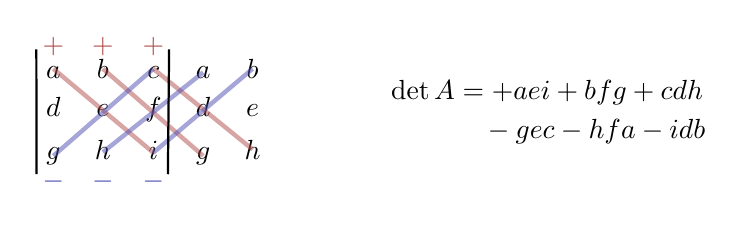
\begin{tikzpicture}[ampersand replacement=\&]
      \matrix[
        matrix of math nodes,
        column sep=2mm,
      ] (sarrus) {
        a\vphantom{b} \& b \& c\vphantom{b} \& a \& b \\
        d \& e \& f \& d \& e                         \\
        g \& h\vphantom{g} \& i\vphantom{g} \& g \& h \\
      };

      \draw[red!40!gray, ultra thick, opacity=.5]
      (sarrus-1-1.center) -- (sarrus-3-3.center)
      (sarrus-1-2.center) -- (sarrus-3-4.center)
      (sarrus-1-3.center) -- (sarrus-3-5.center)
      ;

      \draw[blue!40!gray, ultra thick, opacity=.5]
      (sarrus-3-1.center) -- (sarrus-1-3.center)
      (sarrus-3-2.center) -- (sarrus-1-4.center)
      (sarrus-3-3.center) -- (sarrus-1-5.center)
      ;

      \draw[black, thick]
      (sarrus-1-1.north west) -- (sarrus-3-1.south west)
      (sarrus-1-3.north east) -- (sarrus-3-3.south east)
      ;

      \foreach \i in {1,2,3}{
          \node[above=-2.0mm, red!40!gray] at (sarrus-1-\i.north) {$+$};
          \node[below=-1.5mm, blue!40!gray] at (sarrus-3-\i.south) {$-$};
        }

      \node[] at (5,.25) {$\det \rmat A = + aei + bfg + cdh$};
      \node[] at (5,-.25) {$\phantom{\det \rmat A =} - gec - hfa - idb$};
    \end{tikzpicture}
  \end{center}
\end{blueBox}

\begin{definition}[Mátrix rangja]
  A mátrix rangjának nevezzük az oszlopvektorai közül a lineárisan függetlenek
  maximális számát.
\end{definition}

\begin{theorem}[Mátrixok rangszámának tétele]
  Egy mátrix rangja megegyezik maximális el nem tűnő aldeterminánsának
  rendjével.
\end{theorem}

\begin{note}
  A mátrix rangja elemi mátrix átalakítások során nem változik:
  \begin{itemize}
    \item tetszőleges sorát vagy oszlopát egy 0-tól különböző számmal
          megszorozzuk,
    \item tetszőleges sorát vagy oszlopát felcseréljük,
    \item tetszőleges sorához vagy oszlopához egy másik tetszőleges sorát vagy
          oszlopát adjuk.
  \end{itemize}
\end{note}

\begin{note}
  Ha egy kvadratikus (négyzetes) mátrix determinánsa nem zérus, akkor rangja
  maximális.
  $$
    \rmat A \in \mathcal M_{n \times n}
    \land
    \det \rmat A \neq 0
    \quad \Rightarrow \quad
    \rg \rmat A = n
  $$
\end{note}

\begin{note}
  Egy $m \times n$-es mátrix rangja nem lehet nagyobb, mint az $m$ és az $n$
  közül a kisebbik érték. Ha a mátrix rangja maximális, akkor az $m$ és az $n$
  közül a kisebbik érték a rang.
  $$
    \rmat A \in \mathcal M_{m \times n}
    \quad \Rightarrow \quad
    \rg \rmat A \leq \min\{\; m; n \;\}
  $$
\end{note}

\begin{note}
  Csak a nullmátrixnak lehet 0 rangja.
  % $$
  %   \rg \nmat = 0
  % $$
\end{note}

\begin{example}
  Határozzuk meg az $\rmat A = \begin{bmatrix}
      1 & 2 & 3 \\
      3 & 2 & 1 \\
      2 & 1 & 3
    \end{bmatrix}$ mátrix rangját a definíció segítségével!

  Vizsgáljuk meg, hogy oszlopvektorai lineárisan függetlenek-e, vagyis
  határozzuk meg a mátrix determinánsát:
  $$
    \det \rmat A = \begin{vmatrix}
      1 & 2 & 3 \\
      3 & 2 & 1 \\
      2 & 1 & 3
    \end{vmatrix}
    = 1 \cdot 2 \cdot 3
    + 2 \cdot 1 \cdot 2
    + 3 \cdot 3 \cdot 1
    - 3 \cdot 2 \cdot 3
    - 1 \cdot 1 \cdot 1
    - 3 \cdot 2 \cdot 3
    = -12
    \text.
  $$
  Mivel a determináns értéke nem zérus, az $\rmat A$ mátrix rangja maximális,
  azaz $\rg \rmat A = 3$.
\end{example}

\begin{example}
  Határozzuk meg az $\rmat A = \begin{bmatrix}
      1 & 2 & 3 \\
      3 & 2 & 1 \\
      2 & 1 & 3
    \end{bmatrix}$ mátrix rangját a tétel segítségével!

  A mátrix rangja a legnagyobb el nem tűnő alderermináns rendje:
  \begin{alignat*}{9}
    \rmat A_1
     & = \begin{bmatrix}
           1
         \end{bmatrix}
     & \quad \rightarrow \quad
     & \det \rmat A_1 = 1
    \text,
    \\
    \rmat A_2
     & = \begin{bmatrix}
           1 & 2 \\
           3 & 2
         \end{bmatrix}
     & \quad \rightarrow \quad
     & \det \rmat A_2 = 1 \cdot 2 - 3 \cdot 2 = -4
    \text,
    \\
    \rmat A_3
     & = \begin{bmatrix}
           1 & 2 & 3 \\
           3 & 2 & 1 \\
           2 & 1 & 3
         \end{bmatrix}
     & \quad \rightarrow \quad
     & \det \rmat A_3 = \dots = -12
    \text.
  \end{alignat*}
  Mivel a legnagyobb el nem tűnő aldetermináns rendje 3, ezért az $\rmat A$
  mátrix rangja 3.
\end{example}

\begin{example}
  \newcolumntype{x}[1]{>{\centering\arraybackslash\hspace{0pt}}p{#1}}
  \newcolumntype{F}[1]{>{$}x{#1}<{$}}
  \newenvironment{bamatrix}[2]{\left[\begin{array}{*{#1}{F{#2}}}}{\end{array}\right]}
  Határozzuk meg az $\rmat A = \begin{bmatrix}
      1 & 2 & 3 \\
      3 & 2 & 1 \\
      2 & 1 & 3
    \end{bmatrix}$ mátrix rangját elemi átalakítások segítségével!

  \begin{align*}
    \rg \rmat A
     & = \rg
    \begin{bamatrix}{4}{5.5mm}
      1 & 2 & 3 \\
      3 & 2 & 1 \\
      2 & 1 & 3
    \end{bamatrix}
    \;
    \begin{matrix}
      \\(-3S_1)\\(-2S_1)
    \end{matrix}
    \\
     & = \rg
    \begin{bamatrix}{4}{5.5mm}
      1 & 2 & 3 \\
      0 & -4 & -8 \\
      0 & -3 & -3
    \end{bamatrix}
    \;
    \begin{matrix}
      \\\div(-4)\\
    \end{matrix}
    \\
     & = \rg
    \begin{bamatrix}{4}{5.5mm}
      1 & 2 & 3 \\
      0 & 1 & 2 \\
      0 & -3 & -3
    \end{bamatrix}
    \;
    \begin{matrix}
      \\(-2S_2)\\(+3S_2)
    \end{matrix}
    \\
     & = \rg
    \begin{bamatrix}{4}{5.5mm}
      1 & 0 & -1 \\
      0 & 1 & 2 \\
      0 & 0 & 3
    \end{bamatrix}
    \;
    \begin{matrix}
      \\\\\div 3
    \end{matrix}
    \\
     & = \rg
    \begin{bamatrix}{4}{5.5mm}
      1 & 0 & -1 \\
      0 & 1 & 2 \\
      0 & 0 & 1
    \end{bamatrix}
    \;
    \begin{matrix}
      (+S_3) \\(-2S_3)\\
    \end{matrix}
    \\
     & = \rg
    \begin{bamatrix}{4}{5.5mm}
      1 & 0 & 0 \\
      0 & 1 & 0 \\
      0 & 0 & 1
    \end{bamatrix}
    = 3
  \end{align*}
\end{example}

\begin{definition}[Reguláris és szinguláris mátrix]
  Egy kvadratikus mátrixot \textbf{regulárisnak} mondunk, ha
  determinánsa nem zérus.

  Ha a kvadratikus mátrix determinánsa 0, \textbf{szinguláris} mátrixról
  beszélünk.
\end{definition}

\begin{definition}[Mátrix inverze]
  Az $\rmat A \in \mathcal M_{n \times n}$ mátrix inverzét az $\rmat A^{-1}$
  jelöli, és az a mátrix, melyre $\rmat A \cdot \rmat A^{-1} = \imat$
  teljesül.
\end{definition}

\begin{note}
  Egy szinguláris mátrixnak nem létezik inverze.
\end{note}

\begin{blueBox}
  Reguláris mátrix inverze egyértelmű. Ha $\rmat A \in \mathcal M_{n \times n}$,
  akkor
  $$
    \rmat A^{-1} := \frac{\adj \rmat A}{\det \rmat A}
    \text.
  $$

  Egy $2 \times 2$-es mátrix adjugáltja:
  $$
    \rmat A = \begin{bmatrix}
      a & b \\
      c & d
    \end{bmatrix}
    \quad
    \Rightarrow
    \quad
    \adj \rmat A = \begin{bmatrix}
      d  & -b \\
      -c & a
    \end{bmatrix}
  $$
\end{blueBox}

\begin{example}
  Határozzuk meg az $\rmat A = \begin{bmatrix}
      1 & 2 \\
      3 & 4
    \end{bmatrix}$ mátrix inverzét!

  A mátrix determinánsa:
  $$
    \det \rmat A = 1 \cdot 4 - 3 \cdot 2 = -2
    \text.
  $$
  A mátrix adjugáltja:
  $$
    \adj \rmat A = \begin{bmatrix}
      4  & -2 \\
      -3 & 1
    \end{bmatrix}
    \text.
  $$
  Ezek alapján az $\rmat A$ mátrix inverze:
  $$
    \rmat A^{-1} = \frac{1}{-2} \cdot \begin{bmatrix}
      4  & -2 \\
      -3 & 1
    \end{bmatrix}
    = \begin{bmatrix}
      -2  & 1    \\
      3/2 & -1/2
    \end{bmatrix}
    \text.
  $$
\end{example}

\begin{blueBox}
  Egy $3 \times 3$-as mátrix adjugáltja:
  $$
    \rmat A = \begin{bmatrix}
      a_{11} & a_{12} & a_{13} \\
      a_{21} & a_{22} & a_{23} \\
      a_{31} & a_{32} & a_{33}
    \end{bmatrix}
    \quad
    \Rightarrow
    \quad
    \adj \rmat A = \begin{bmatrix}
      + \begin{vmatrix}
          a_{22} & a_{23} \\
          a_{32} & a_{33}
        \end{vmatrix}
       &
      - \begin{vmatrix}
          a_{12} & a_{13} \\
          a_{32} & a_{33}
        \end{vmatrix}
       &
      +\begin{vmatrix}
         a_{12} & a_{13} \\
         a_{22} & a_{23}
       \end{vmatrix}
      \\
      - \begin{vmatrix}
          a_{21} & a_{23} \\
          a_{31} & a_{33}
        \end{vmatrix}
       &
      + \begin{vmatrix}
          a_{11} & a_{13} \\
          a_{31} & a_{33}
        \end{vmatrix}
       &
      - \begin{vmatrix}
          a_{11} & a_{13} \\
          a_{21} & a_{23}
        \end{vmatrix}
      \\
      + \begin{vmatrix}
          a_{21} & a_{22} \\
          a_{31} & a_{32}
        \end{vmatrix}
       &
      - \begin{vmatrix}
          a_{11} & a_{12} \\
          a_{31} & a_{32}
        \end{vmatrix}
       &
      +\begin{vmatrix}
         a_{11} & a_{12} \\
         a_{21} & a_{22}
       \end{vmatrix}
    \end{bmatrix}
  $$
\end{blueBox}

\begin{note}
  $3 \times 3$-as mátrix adjugáltjának felírásához érdemes először a
  transzponáltját felírni, például:
  $$
    \rmat A = \begin{bmatrix}
      a_{11} & a_{21} & a_{31} \\
      a_{12} & a_{22} & a_{32} \\
      a_{13} & a_{23} & a_{33}
    \end{bmatrix}
    \quad \Rightarrow \quad
    \rmat A^\T = \begin{bmatrix}
      a_{11} & a_{12} & a_{13} \\
      a_{21} & a_{22} & a_{23} \\
      a_{31} & a_{32} & a_{33}
    \end{bmatrix}
  $$

  Az adjugált $i$-edik sorában és $j$-edik oszlopában elhelyezkező $\alpha_{ij}$
  elemét a letakarós módszer segítségével határozhatjuk meg.

  Az adjugált első sorának elemei:
  \begin{center}
    \begin{tikzpicture}[ampersand replacement=\&]
      \matrix[
      matrix of math nodes,
      column sep=2mm,
      ] (m) {
      {}^+ a_{11} \& {}^- a_{21} \& {}^+ a_{31} \\
      {}^- a_{12} \& {}^+ a_{22} \& {}^- a_{32}      \\
      {}^+ a_{13} \& {}^- a_{23} \& {}^+ a_{33}      \\
      };

      \draw[primaryColor, line width=5mm, opacity=.5]
      (m-1-1.west) -- (m-1-3.east)
      ;
      \draw[primaryColor, line width=8mm, opacity=.5]
      (m-1-1.north) -- (m-3-1.south)
      ;

      \draw[black, thick]
      (m-1-1.north west) -- (m-3-1.south west)
      (m-1-3.north east) -- (m-3-3.south east)
      ;

      \node at (0,-2.25) {$\alpha_{11} = + \begin{vmatrix}
            a_{22} & a_{23} \\
            a_{32} & a_{33}
          \end{vmatrix}$};

      \begin{scope}[xshift=5cm]
        \matrix[
        matrix of math nodes,
        column sep=2mm,
        ] (m) {
        {}^+ a_{11} \& {}^- a_{21} \& {}^+ a_{31} \\
        {}^- a_{12} \& {}^+ a_{22} \& {}^- a_{32}      \\
        {}^+ a_{13} \& {}^- a_{23} \& {}^+ a_{33}      \\
        };

        \draw[secondaryColor, line width=5mm, opacity=.5]
        (m-1-1.west) -- (m-1-3.east)
        ;
        \draw[secondaryColor, line width=8mm, opacity=.5]
        (m-1-2.north) -- (m-3-2.south)
        ;

        \draw[black, thick]
        (m-1-1.north west) -- (m-3-1.south west)
        (m-1-3.north east) -- (m-3-3.south east)
        ;

        \node at (0,-2.25) {$\alpha_{12} = - \begin{vmatrix}
              a_{12} & a_{32} \\
              a_{13} & a_{33}
            \end{vmatrix}$};
      \end{scope}

      \begin{scope}[xshift=10cm]
        \matrix[
        matrix of math nodes,
        column sep=2mm,
        ] (m) {
        {}^+ a_{11} \& {}^- a_{21} \& {}^+ a_{31} \\
        {}^- a_{12} \& {}^+ a_{22} \& {}^- a_{32}      \\
        {}^+ a_{13} \& {}^- a_{23} \& {}^+ a_{33}      \\
        };

        \draw[primaryColor, line width=5mm, opacity=.5]
        (m-1-1.west) -- (m-1-3.east)
        ;
        \draw[primaryColor, line width=8mm, opacity=.5]
        (m-1-3.north) -- (m-3-3.south)
        ;

        \draw[black, thick]
        (m-1-1.north west) -- (m-3-1.south west)
        (m-1-3.north east) -- (m-3-3.south east)
        ;

        \node at (0,-2.25) {$\alpha_{13} = + \begin{vmatrix}
              a_{12} & a_{22} \\
              a_{13} & a_{23}
            \end{vmatrix}$};
      \end{scope}
    \end{tikzpicture}
  \end{center}
  A többi elem hasonló módszerrel számolható.
\end{note}

\begin{example}
  Határozzuk meg az $\rmat A = \begin{bmatrix}
      1 & 2 & 3 \\
      3 & 4 & 5 \\
      5 & 6 & 8 \\
    \end{bmatrix}$ mátrix inverzét!

  A mátrix determinánsa:
  $$
    \det \rmat A
    = 1 \cdot 4 \cdot 8
    + 2 \cdot 5 \cdot 5
    + 3 \cdot 3 \cdot 6
    - 3 \cdot 4 \cdot 5
    - 6 \cdot 5 \cdot 1
    - 8 \cdot 2 \cdot 3
    = -2
    \text.
  $$
  A mátrix transzponáltja:
  $$
    \rmat A^\T = \begin{bmatrix}
      1 & 3 & 5 \\
      2 & 4 & 6 \\
      3 & 5 & 8
    \end{bmatrix}
    \text.
  $$
  A mátrix adjugáltja:
  $$
    \adj \rmat A = \begin{bmatrix}
      + \begin{vmatrix}
          4 & 5 \\
          6 & 8
        \end{vmatrix}
       &
      - \begin{vmatrix}
          2 & 3 \\
          6 & 8
        \end{vmatrix}
       &
      + \begin{vmatrix}
          2 & 3 \\
          4 & 5
        \end{vmatrix}
      \\
      - \begin{vmatrix}
          3 & 5 \\
          5 & 8
        \end{vmatrix}
       &
      + \begin{vmatrix}
          1 & 3 \\
          5 & 8
        \end{vmatrix}
       &
      - \begin{vmatrix}
          1 & 3 \\
          3 & 5
        \end{vmatrix}
      \\
      + \begin{vmatrix}
          3 & 4 \\
          5 & 6
        \end{vmatrix}
       &
      - \begin{vmatrix}
          1 & 2 \\
          5 & 6
        \end{vmatrix}
       &
      + \begin{vmatrix}
          1 & 2 \\
          3 & 4
        \end{vmatrix}
    \end{bmatrix}
    =
    \begin{bmatrix}
      2  & 2  & -2 \\
      1  & -7 & 4  \\
      -2 & 4  & -2
    \end{bmatrix}
    \text.
  $$
  A mátrix inverze:
  $$
    \rmat A^{-1} = \frac{1}{-2} \cdot \begin{bmatrix}
      2  & 2  & -2 \\
      1  & -7 & 4  \\
      -2 & 4  & -2
    \end{bmatrix}
    = \begin{bmatrix}
      -1   & -1  & 1  \\
      -1/2 & 7/2 & -2 \\
      1    & -2  & 1
    \end{bmatrix}
    \text.
  $$
\end{example}

\begin{blueBox}
  \sftitle{Inverz meghatározása Gauss-Jordan eliminációval:}

  Egy $\rmat A$ reguláris mátrix inverzés Gauss-Jordan eliminációval
  is meghatározhatjuk. A módszer során az $(\rmat A | \imat)$ mátrixot
  sorműveletek segítségével olyan módon alakítjuk át, hogy ahol eredetileg
  $\rmat A$ állt, ott az egységmátrix jelenjen meg. Az átalakított mátrix
  másik felében az $\rmat A^{-1}$ mátrix fog szerepelni.
\end{blueBox}

\begin{example}
  Határozzuk meg az $\rmat A = \begin{bmatrix}
      1 & 2 \\
      3 & 4
    \end{bmatrix}$ mátrix inverzét!
  \newcolumntype{x}[1]{>{\centering\arraybackslash\hspace{0pt}}p{#1}}
  \newcolumntype{F}[1]{>{$}x{#1}<{$}}
  \begin{align*}
     & \left[\begin{array}{F{9mm}F{9mm}|F{9mm}F{9mm}}
                 1 & 2 & 1 & 0 \\
                 3 & 4 & 0 & 1
               \end{array}\right]\begin{matrix}\\(-3S_1)\,\end{matrix}
    \\
     & \left[\begin{array}{F{9mm}F{9mm}|F{9mm}F{9mm}}
                 1 & 2  & 1  & 0 \\
                 0 & -2 & -3 & 1
               \end{array}\right]\begin{matrix}\\\div(-2)\,\end{matrix}
    \\
     & \left[\begin{array}{F{9mm}F{9mm}|F{9mm}F{9mm}}
                 1 & 2 & 1   & 0    \\
                 0 & 1 & 3/2 & -1/2
               \end{array}\right]\begin{matrix}(-2S_2)\\\,\end{matrix}
    \\
     & \left[\begin{array}{F{9mm}F{9mm}|F{9mm}F{9mm}}
                 1 & 0 & -1/2 & 1/2  \\
                 0 & 1 & 3/2  & -1/2
               \end{array}\right]
  \end{align*}
\end{example}

% \begin{blueBox}


%   \textbf{1. módszer - definíció alapján:} Az inverz meghatározása a mátrix determinánsának segítségével.
%   \[
%     \textbf{A}^{-1} = \frac{1}{\text{det}(\textbf{A})} \cdot \text{adj}(\textbf{A})
%   \]
%   \textbf{2. módszer - Gauss-Jordan módszer:} Az inverz meghatározása a mátrix sorai és oszlopai alapján
%   \begin{enumerate}
%     \item \textbf{Mátrix előkészítése:} Írd fel a mátrixot bővített alakban.
%     \item \textbf{Főelemek kiválasztása:}
%           \begin{itemize}
%             \item Az aktuális főelemet állítsd \(1\)-re (osztással).
%             \item Nullázd ki az oszlop többi elemét (fölötte és alatta).
%           \end{itemize}
%     \item \textbf{Redukált lépcsős alak (Row echelon form):} Ismételd a fenti lépéseket, amíg minden oszlopban lépcsőzetesen emelkedő \(1\)-eseket kapsz.
%     \item \textbf{Megoldás:} A rangot vagy az egyenletrendszer megoldását a mátrix egyszerűsített alakjából olvasd ki.
%   \end{enumerate}

% \end{blueBox}

\clearpage
\subsection{Feladatok}

\begin{enumerate}
  \item Egy síkon vannak-e az $A(2,3,-4)$, $B(3,-1,-6)$, $C(-1,5,2)$ és
        $D(2,1,-4)$ pontok?

  \item Számolja ki azalábbi mátrixok determinánsát Sarrus-szabállyal!
        $$
          \rmat A =
          \begin{bmatrix}
            4 & 9 & 2 \\
            3 & 5 & 7 \\
            8 & 1 & 6
          \end{bmatrix}
          \qquad
          \rmat B =
          \begin{bmatrix}
            3 & 5 & 7 \\
            5 & 6 & 3 \\
            2 & 1 & 4
          \end{bmatrix}
          \qquad
          \rmat C =
          \begin{bmatrix}
            8  & 4 & 3  \\
            -5 & 6 & -2 \\
            7  & 9 & -8
          \end{bmatrix}
          \qquad
          \rmat D =
          \begin{bmatrix}
            4 & -3 & 0 \\
            2 & -1 & 2 \\
            1 & 5  & 7
          \end{bmatrix}
        $$

  \item Adja meg az azalábbi mátrixok rangját!
        \begin{alignat*}{9}
          \rmat A & =
          \begin{bmatrix}
            1 & 2 & 3 \\
            3 & 2 & 1 \\
            2 & 1 & 3
          \end{bmatrix}
          \hspace{5cm}
                  & \rmat B & =
          \begin{bmatrix}
            1  & 3  & -2 \\
            -2 & -6 & 4  \\
            -1 & -3 & 2
          \end{bmatrix}
          \\
          \rmat C & =
          \begin{bmatrix}
            1  & 1 & 2  & 3 \\
            2  & 4 & 5  & 2 \\
            -1 & 1 & -1 & 0
          \end{bmatrix}
          \qquad
                  & \rmat D & =
          \begin{bmatrix}
            1 & 2 & 3 & 4 & 5 \\
            2 & 3 & 4 & 5 & 6 \\
            5 & 6 & 7 & 8 & 9 \\
            4 & 5 & 6 & 7 & 8
          \end{bmatrix}
        \end{alignat*}


  \item Vizsgálja az $\rmat A$ mátrix rangját $x$ függvényében!
        $$
          \rmat A = \begin{bmatrix}
            1 & -1 & -3 & 3 \\
            x & 4  & 10 & 1 \\
            1 & 7  & 17 & 3 \\
            2 & 2  & 4  & 1
          \end{bmatrix}
        $$

  \item Számítsa ki az alábbi mátrixok inverzét!
        $$
          \rmat A =
          \begin{bmatrix}
            1 & 2 \\
            3 & 4
          \end{bmatrix}
          \qquad
          \rmat B =
          \begin{bmatrix}
            4 & 5 \\
            2 & 6
          \end{bmatrix}
          \qquad
          \rmat C =
          \begin{bmatrix}
            1 & 3 & 3 \\
            1 & 3 & 4 \\
            1 & 4 & 3
          \end{bmatrix}
          \qquad
          \rmat D =
          \begin{bmatrix}
            1 & 2 & 3 \\
            3 & 2 & 1 \\
            2 & 1 & 3
          \end{bmatrix}
        $$

  \item Milyen $k$ érték esetén lesz invertálható az alábbi mátrix?
        $$
          \begin{bmatrix}
            k-1 & 2   \\
            2   & k-1
          \end{bmatrix}
        $$

  \item Határozza meg az ismeretlenekeket az alábbi mátrixegyenletben!
        $$
          \begin{bmatrix}
            x  & 5 \\
            -3 & z
          \end{bmatrix}
          \begin{bmatrix}
            7 & y \\
            0 & 6
          \end{bmatrix}
          =
          \begin{bmatrix}
            -14 & 8 \\
            w   & 3
          \end{bmatrix}
        $$

  \item Adottak az $\rmat A$, $\rmat B$ és $\rmat C$ mátrixok. Oldja meg az
        alábbi mátrixegyenletet!
        $$
          \rmat A = \begin{bmatrix}
            4 & 3 \\
            1 & 1
          \end{bmatrix}
          \qquad
          \rmat B = \begin{bmatrix}
            1 & 2 \\
            3 & 4
          \end{bmatrix}
          \qquad
          \rmat C = \begin{bmatrix}
            1 & -1 \\
            2 & -3
          \end{bmatrix}
          \qquad \Rightarrow \qquad
          \rmat A \rvec x + \rmat C = 2\rmat B \rmat C \rvec x
        $$

  \item Számítsa ki az alábbi, komplex elemű mátrix rangját!
        $$
          \begin{bmatrix}
            1  & 2i & 1+2i    \\
            3  & i  & 3-i     \\
            4i & -3 & -1 + 4i
          \end{bmatrix}
        $$
\end{enumerate}


\end{document}